\chapter{Partículas, ondas y energía de resolución}

\section{¿Partículas o campos?}

¿De qué trata la física de partículas? De partículas---, pero esa respuesta plantea de inmediato una antigua pregunta: ¿es discreta la naturaleza? Aquí, discreto significa que la materia está formada por unidades separadas e indivisibles, no que sea diplomática. La palabra griega \emph{átomo} significa indivisible, aunque los objetos que ahora llamamos átomos puedan dividirse. Por ahora, \emph{partícula} será el nombre genérico de una unidad discreta.

La imagen opuesta es la de un continuo. En ese caso, la materia no es un conjunto de partes separadas, sino una distribución continua por el espacio. Su lenguaje natural es el de los campos. Un campo es una función de la posición: la densidad de un material es un campo, y los campos eléctrico y magnético también lo son. Estos últimos determinan cómo se mueven las partículas cargadas, pero, en la concepción clásica, los propios campos están distribuidos continuamente por el espacio.

No conviene insistir demasiado en el orden histórico de estas ideas. La secuencia es útil porque muestra la lógica del argumento, no porque proporcione una cronología fiable. El vocabulario de las partículas incluye átomos, moléculas, colisiones y objetos localizados; el del continuo incluye campos y propiedades que varían continuamente. ¿Cuál de las dos imágenes es correcta? La mecánica cuántica impide que cualquiera de ellas sea completamente correcta, pero también impide que sea completamente incorrecta.

La exposición será en parte autocontenida, aunque los argumentos posteriores recurren a la mecánica cuántica, la mecánica clásica, la relatividad especial y el electromagnetismo. La pregunta inmediata es más sencilla: ¿qué convenció primero a la gente de que la materia es realmente discreta?

\section{Evidencia química de la materia discreta}

La primera evidencia sólida provino, al menos en esta exposición lógica, de la química y no de la física. La distinción es artificial: la química es, en gran medida, la física de los átomos y las moléculas. Dalton comparó las masas de cantidades iguales de moléculas de distintas sustancias. Determinar que las muestras contenían el mismo número de moléculas ya era, por sí solo, un problema importante. Aquí aparece el nombre de Avogadro: un mol contiene el número de Avogadro de moléculas. Para comparar muestras que contenían el mismo número de moléculas no hacía falta conocer el valor exacto de ese número.

El patrón llamativo era que las masas molares eran aproximadamente múltiplos enteros de la masa molar del hidrógeno. Los multiplicadores no solían ser \(3/2\), \(\pi\) ni números reales arbitrarios, sino números cercanos a enteros. El carbono-12, por ejemplo, tiene aproximadamente doce veces las unidades de masa representadas por el hidrógeno. Esto sugiere con fuerza una estructura formada por bloques repetidos de masa casi idéntica.

La explicación moderna disipa el misterio. Los átomos ordinarios contienen protones, neutrones y electrones. La masa de un electrón es apenas una dosmilésima parte, aproximadamente, de la de un protón o un neutrón, así que los electrones contribuyen poco a la masa atómica. Los protones y neutrones aportan casi toda esa masa, y sus masas difieren en mucho menos de un uno por ciento. Como el núcleo del hidrógeno ordinario consta de un protón, la masa de un átomo o una molécula es aproximadamente un múltiplo entero de una masa nuclear del orden de la del hidrógeno. La afirmación es solo aproximada: las masas del protón y el neutrón no son idénticas, y los electrones contribuyen un poco. Aun así, el patrón casi entero revela la existencia de constituyentes discretos.

Más adelante se entendió que las moléculas son combinaciones de átomos. La química del siglo XIX identificó alrededor de un centenar de tipos de átomos y los organizó como elementos; en el recuento elemental, unos noventa y dos se encuentran de forma natural, aunque al incluir los isótopos aparecen más distinciones. La tabla periódica no es periódica en el sentido ingenuo de repetir bloques iguales sin más, pero permitió organizar esas especies separadas. En aquella etapa, los propios elementos parecían ser los bloques de construcción elementales. El trabajo de Einstein de 1905 aportó una manera cuantitativa de establecer con mucha más contundencia la teoría molecular de la materia, pero la evidencia química ya había hecho convincente la imagen atómica.

Hacia finales del siglo XIX, este aparente punto final dejó de serlo. Se descubrió el electrón y la radiactividad reveló fenómenos que no cabían en la imagen de los elementos como entidades elementales. La radiactividad ya contenía, en miniatura, muchas de las preguntas que después serían propias de la física nuclear y de partículas.

\section{Radiactividad y haces separados}

La atribución y la cronología exactas son inciertas. Se suele asociar, con cautela, a Becquerel con la observación de que un material radiactivo, colocado por casualidad cerca de una placa fotográfica, la afectaba como si una radiación invisible la hubiera iluminado. En lugar de considerar que la placa velada simplemente se había estropeado, cabía preguntarse qué había llegado hasta ella. La extensa labor posterior de Marie Curie también forma parte de esta historia, pero no hace falta precisar el reparto de los primeros descubrimientos para entender la lógica experimental.

Coloca el material en el interior de un bloque grueso de plomo y deja un canal estrecho que apunte hacia una placa fotográfica. El plomo es útil porque es denso, mientras que el canal colima lo que logra escapar. En vez de una exposición difusa, la placa revela una mancha localizada, lo que sugiere un haz dirigido. En este sentido lógico, se trata del primer haz de partículas, aunque en esta etapa todavía se desconoce la naturaleza del haz.

Haz pasar ahora la emisión colimada por un campo magnético perpendicular al plano de las trayectorias. La exposición se separa en tres ramas. Una sigue sin desviarse. Dos se curvan en sentidos opuestos y en distinta medida. La fuerza magnética invierte su sentido cuando cambia el signo de la carga, así que las ramas que se curvan en sentidos opuestos se comportan como radiaciones con cargas opuestas; la rama recta se comporta como radiación neutra.\footnote{El esquema reconstruye el diagrama desarrollado en el vídeo de la clase entre 00:14:34 y 00:19:31.}

\begin{figure}[h]
\centering
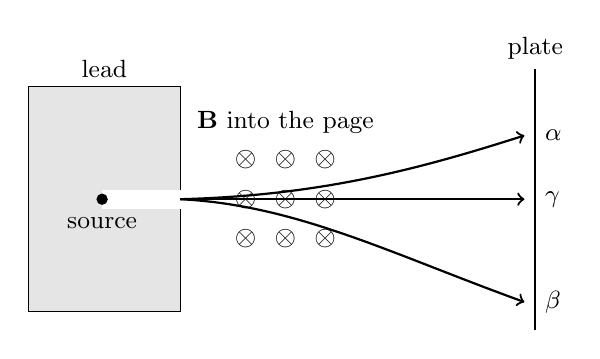
\begin{tikzpicture}[scale=0.92]
\draw[fill=gray!20] (0,-1.55) rectangle (2.1,1.55);
\draw[fill=white,draw=none] (1.02,-0.13) rectangle (2.12,0.13);
\draw[fill=black] (1.02,0) circle (0.07);
\node[below] at (1.02,-0.12) {\small source};
\node[above] at (1.05,1.55) {\small lead};
\foreach \x in {3.0,3.55,4.1}
  \foreach \y in {-0.55,0,0.55}
    \node at (\x,\y) {\(\otimes\)};
\node[above] at (3.55,0.78) {\small \(\mathbf B\) into the page};
\draw[thick] (7,-1.8) -- (7,1.8);
\node[above] at (7,1.8) {\small plate};
\draw[thick,->] (2.1,0) -- (6.85,0);
\draw[thick,->] (2.1,0) .. controls (4.0,0.05) and (5.35,0.40) .. (6.85,0.88);
\draw[thick,->] (2.1,0) .. controls (3.7,-0.08) and (5.0,-0.75) .. (6.85,-1.42);
\node[right] at (7,0.88) {\small \(\alpha\)};
\node[right] at (7,0) {\small \(\gamma\)};
\node[right] at (7,-1.42) {\small \(\beta\)};
\end{tikzpicture}
\caption{Un haz radiactivo colimado en un campo magnético transversal. El componente neutro no se desvía, mientras que los componentes con cargas opuestas se curvan en sentidos opuestos y en distinta medida.}
\end{figure}

Los tres componentes recibieron los nombres de alfa, beta y gamma. En términos modernos,
\begin{equation}
\begin{aligned}
\beta\text{-radiation} &= \text{electrons},\\
\alpha\text{-radiation} &= \text{helium nuclei},\\
\gamma\text{-radiation} &= \text{photons}.
\end{aligned}
\end{equation}
Una partícula alfa contiene dos protones y dos neutrones, lo que explica su número másico cuatro. Por tanto, en la secuencia aproximada de números enteros de Dalton, el helio habría ocupado el número cuatro: cuatro unidades nucleares del orden de la masa del hidrógeno. Los rayos beta son los electrones con carga negativa que ya se conocían por los experimentos con rayos catódicos. Los rayos gamma no tienen carga eléctrica.

Con una fuente suficientemente diluida y un detector capaz de resolver llegadas individuales, la exposición que parecía continua se convierte en una sucesión de eventos separados: destello, destello, destello. Lo mismo puede hacerse con la radiación beta, alfa y gamma. Un contador Geiger ofrece la imagen adecuada, tanto si los primeros aparatos se usaron exactamente en ese régimen como si no. Cada componente llega en paquetes discretos. Los rayos gamma siguen planteando un enigma: son neutros y, aun así, se detectan evento por evento. La radiación gamma es luz de energía muy alta, y Planck y, en especial, Einstein relacionaron la luz con los cuantos. Sin embargo, antes de afrontar esa conclusión, hay que tomar en serio la evidencia clásica de que la luz es una onda.

\section{El carácter ondulatorio clásico de la luz}

Desde el punto de vista clásico, la luz era el ejemplo más contundente de continuidad. Consiste en campos eléctricos y magnéticos que se propagan como ondas continuas. Newton había favorecido una imagen corpuscular, pero los experimentos con ondas la desplazaron. Al agitar una carga se produce radiación electromagnética. Una antena macroscópica puede emitir ondas de radio, microondas, radiación infrarroja, luz visible o radiación ultravioleta; una carga que se mueve dentro de un átomo también actúa como antena. La radiación emitida puede exponer una placa fotográfica.

Una sola abertura ofrece un primer indicio del comportamiento ondulatorio. Si la luz fuera un flujo de balas, cabría esperar que una abertura pequeña produjera una mancha nítida y colimada. En cambio, la iluminación se extiende en una región difusa. Sin embargo, la propagación por sí sola no es concluyente, pues podría imaginarse que las partículas se desvían por fuerzas en el borde de la abertura.

Dos aberturas ofrecen una prueba más precisa. Dos flujos de partículas independientes producirían dos manchas superpuestas, quizá con mayor intensidad en la zona de solapamiento. Las ondas se comportan de otro modo. Una cresta procedente de una abertura puede encontrarse con una cresta procedente de la otra y reforzarla; también puede encontrarse con un valle y cancelarse. Por eso la pantalla muestra franjas brillantes y oscuras alternadas, incluidas zonas oscuras que cada abertura iluminaría por sí sola.\footnote{El esquema reconstruye los diagramas de las aberturas y de la interferencia desarrollados en el vídeo de la clase entre 00:25:00 y 00:29:49.}

\begin{figure}[h]
\centering
\resizebox{\linewidth}{!}{%
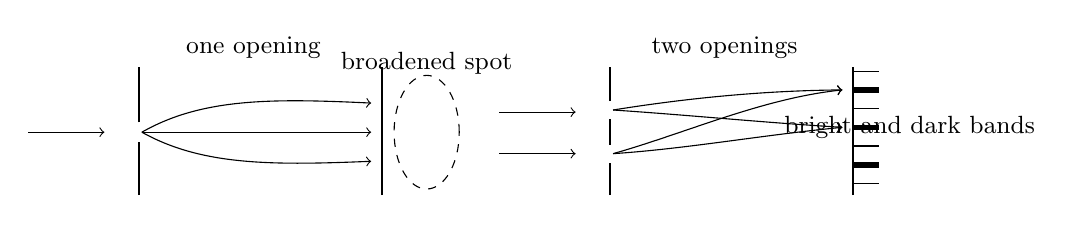
\begin{tikzpicture}[scale=0.88]
\begin{scope}
\draw[->] (-0.3,1.06) -- (0.8,1.06);
\draw[thick] (1.3,0.15) -- (1.3,0.92);
\draw[thick] (1.3,1.20) -- (1.3,2.0);
\draw[thick] (4.8,0.15) -- (4.8,2.0);
\draw[->] (1.34,1.06) .. controls (2.2,1.55) and (3.2,1.55) .. (4.65,1.48);
\draw[->] (1.34,1.06) -- (4.65,1.06);
\draw[->] (1.34,1.06) .. controls (2.2,0.58) and (3.2,0.58) .. (4.65,0.64);
\draw[dashed] (5.45,1.06) ellipse (0.47 and 0.82);
\node at (2.95,2.28) {\small one opening};
\node at (5.45,2.05) {\small broadened spot};
\end{scope}
\begin{scope}[xshift=6.8cm]
\draw[->] (-0.3,1.35) -- (0.8,1.35);
\draw[->] (-0.3,0.75) -- (0.8,0.75);
\draw[thick] (1.3,0.15) -- (1.3,0.62);
\draw[thick] (1.3,0.88) -- (1.3,1.25);
\draw[thick] (1.3,1.51) -- (1.3,2.0);
\draw[thick] (4.8,0.15) -- (4.8,2.0);
\draw[thin] (4.8,0.32) -- (5.18,0.32);
\draw[line width=2pt] (4.8,0.59) -- (5.18,0.59);
\draw[thin] (4.8,0.86) -- (5.18,0.86);
\draw[line width=2pt] (4.8,1.13) -- (5.18,1.13);
\draw[thin] (4.8,1.40) -- (5.18,1.40);
\draw[line width=2pt] (4.8,1.67) -- (5.18,1.67);
\draw[thin] (4.8,1.94) -- (5.18,1.94);
\draw[->] (1.34,0.75) .. controls (2.4,0.82) and (3.5,1.02) .. (4.65,1.13);
\draw[->] (1.34,1.38) .. controls (2.4,1.31) and (3.5,1.20) .. (4.65,1.13);
\draw[->] (1.34,0.75) .. controls (2.4,1.05) and (3.5,1.55) .. (4.65,1.67);
\draw[->] (1.34,1.38) .. controls (2.4,1.55) and (3.5,1.66) .. (4.65,1.67);
\node at (2.95,2.28) {\small two openings};
\node at (5.62,1.13) {\small bright and dark bands};
\end{scope}
\end{tikzpicture}
}
\caption{Una sola abertura produce una imagen ensanchada, mientras que dos aberturas producen interferencia constructiva y destructiva alternada.}
\end{figure}

El mismo efecto es fácil de imaginar en el agua. Mueve dos dedos en la superficie: las ondas circulares se propagan, se refuerzan en algunos lugares y se cancelan en otros. La interferencia, y no la mera propagación, es la señal decisiva del carácter ondulatorio.

Una vez más, la secuencia histórica no es sencilla. En este esquema, Huygens aparece antes que Newton como defensor de la propagación ondulatoria; Thomas Young se asocia con la demostración de la interferencia; y algunos experimentos ópticos del propio Newton admiten una interpretación basada en la interferencia de ondas, aunque él favoreciera los corpúsculos. Los experimentos posteriores de interferencia establecieron sin lugar a dudas razonables el carácter ondulatorio de la luz.

Después, Maxwell identificó qué es lo que oscila. Si una onda luminosa se propaga a lo largo de un eje, su campo eléctrico es transversal a ese eje. Su campo magnético también es transversal y perpendicular al campo eléctrico. El patrón completo se propaga a la velocidad de la luz.\footnote{El esquema reconstruye el diagrama de la onda electromagnética dibujado en el vídeo de la clase en 00:31:08.}

\begin{figure}[h]
\centering
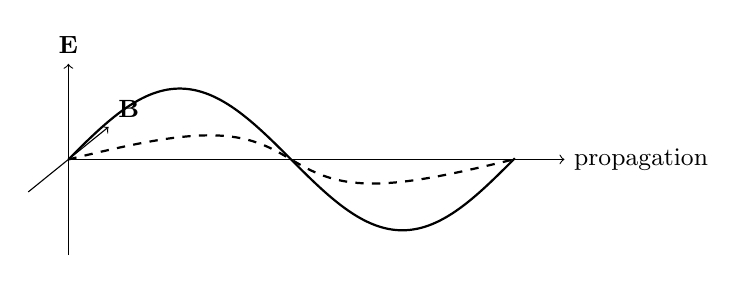
\begin{tikzpicture}[
  scale=0.9,
  x={(1cm,0cm)},
  y={(0cm,1cm)},
  z={(0.42cm,0.34cm)}
]
\draw[->] (0,0,0) -- (7,0,0) node[right] {\small propagation};
\draw[->] (0,-1.35,0) -- (0,1.35,0) node[above] {\small \(\mathbf E\)};
\draw[->] (0,0,-1.35) -- (0,0,1.35) node[above right] {\small \(\mathbf B\)};
\draw[thick,smooth,variable=\x,domain=0:6.3,samples=100]
  plot ({\x},{sin(\x r)},0);
\draw[thick,dashed,smooth,variable=\x,domain=0:6.3,samples=100]
  plot ({\x},0,{sin(\x r)});
\end{tikzpicture}
\caption{En una onda electromagnética, los campos eléctrico y magnético son perpendiculares entre sí y ambos son transversales a la dirección de propagación.}
\end{figure}

La luz visible ordinaria oscila demasiado deprisa para seguir directamente las variaciones alternas de los campos. En una onda de radio extremadamente larga, la oscilación sería correspondientemente más lenta. En ambos casos, la misma geometría de onda transversal produce interferencia.

\section{Longitud de onda, período y frecuencia}

La longitud de onda \(\lambda\) es una distancia espacial: se parte de un punto de la oscilación y se avanza a lo largo de la onda hasta que se repite la misma fase tras un ciclo completo. Se mide en metros, centímetros o cualquier otra unidad de longitud.

Ahora quédate en una posición mientras pasa la onda. El tiempo que tarda en completar un ciclo es el período \(T\). El período de la luz visible es extremadamente corto, del orden de \(10^{-15}\,\mathrm{s}\); a mayor longitud de onda, mayor período, y a menor longitud de onda, menor período.

Durante un período, la onda avanza una longitud de onda, así que una onda de velocidad \(v\) cumple
\begin{equation}
v=\frac{\lambda}{T}.
\end{equation}
Las ondas de agua y de sonido tienen sus propias velocidades de propagación. Para la luz,
\begin{equation}
c=\frac{\lambda}{T}.
\end{equation}
La frecuencia \(f\) es el número de ciclos por unidad de tiempo:
\begin{equation}
f=\frac{1}{T}.
\end{equation}
Por tanto,
\begin{equation}
\lambda f=c.
\end{equation}
La longitud de onda determina la frecuencia, y viceversa.

\begin{figure}[h]
\centering
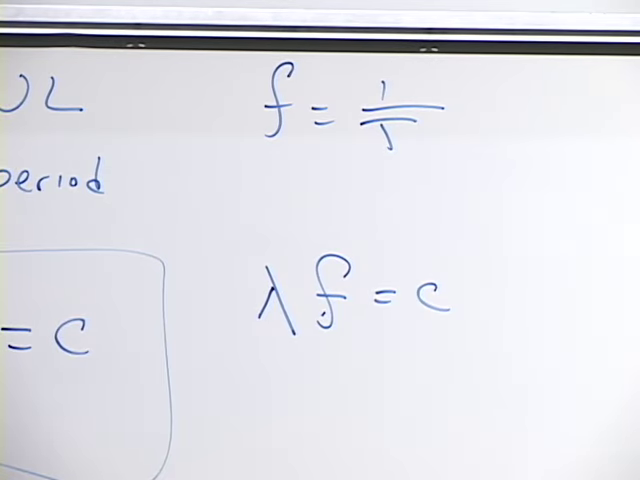
\includegraphics[width=0.68\textwidth]{lecture_01_figure_03.png}
\caption{Para una onda luminosa, \(f=1/T\) y \(\lambda f=c\).}
\lectureframe{00:36:24}
\end{figure}

Los físicos suelen medir la rapidez de oscilación en radianes por segundo, en lugar de ciclos completos por segundo. Imagina un movimiento uniforme en una circunferencia. Si el punto completa \(f\) vueltas cada segundo y cada vuelta contiene \(2\pi\) radianes, su frecuencia angular es
\begin{equation}
\omega=2\pi f,
\qquad
\frac{\omega}{2\pi}=f.
\end{equation}
Por ahora, esto es una definición; más adelante se retomará la cuestión práctica de si reduce el número de factores \(2\pi\).

Al combinar \(f=c/\lambda\) con \(\omega=2\pi f\) se obtiene
\begin{equation}
\omega=\frac{2\pi c}{\lambda},
\qquad
\omega\lambda=2\pi c.
\end{equation}
Para otro tipo de onda, \(c\) se sustituye por la velocidad de propagación de esa onda.

\begin{figure}[h]
\centering
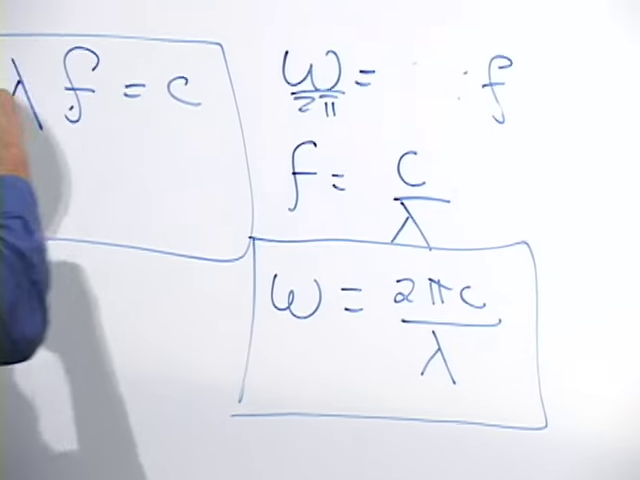
\includegraphics[width=0.68\textwidth]{lecture_01_figure_04.png}
\caption{Para \(\omega=2\pi f\), una onda luminosa cumple \(\omega=2\pi c/\lambda\).}
\lectureframe{00:39:10}
\end{figure}

La radiación electromagnética forma un espectro continuo. En orden de mayor a menor longitud de onda, los nombres convencionales son
\begin{equation}
\begin{aligned}
\text{radio}
&\longrightarrow \text{microwave}
\longrightarrow \text{infrared}
\longrightarrow \text{visible}\\
&\longrightarrow \text{ultraviolet}
\longrightarrow \text{X ray}
\longrightarrow \text{gamma ray}.
\end{aligned}
\end{equation}
La luz visible ocupa solo un intervalo estrecho. Los límites entre las regiones con nombre son convencionales, así que aquí no hace falta dar longitudes de onda divisorias exactas. Las ondas de radio pueden ser extremadamente largas; la radiación gamma ocupa el extremo de longitud de onda muy corta del espectro electromagnético. Ahora la dificultad queda clara: clásicamente, la radiación gamma es una onda de campo continuo, pero se detecta en destellos discretos.

\section{Llegadas discretas y probabilidades ondulatorias}

Las propiedades termodinámicas de la radiación llevaron a Planck y Einstein a la conclusión de que la luz debe tratarse en unidades discretas. Un experimento imaginario hace vívida la idea, pero no pretende describir la ruta histórica real que condujo al descubrimiento.

Ilumina una pantalla con un haz. Con una intensidad normal, se forma una mancha iluminada de aspecto continuo. Coloca en el haz un atenuador parcialmente opaco: la mancha se vuelve más tenue. Aumenta varias veces la atenuación y llega menos luz por unidad de tiempo. Al final, cambia el aspecto. En vez de una mancha continuamente más tenue, el detector registra eventos aislados.\footnote{El esquema reconstruye el experimento de atenuación desarrollado en el vídeo de la clase entre 00:42:32 y 00:45:42.}

\begin{figure}[h]
\centering
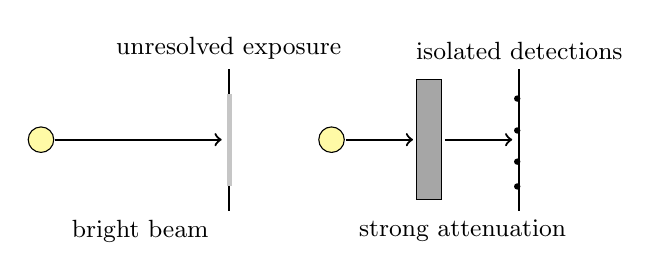
\begin{tikzpicture}[scale=0.9]
\begin{scope}
\draw[fill=yellow!35] (0,0) circle (0.18);
\draw[->,thick] (0.2,0) -- (2.55,0);
\draw[thick] (2.65,-1.0) -- (2.65,1.0);
\node[below] at (1.4,-1.0) {\small bright beam};
\end{scope}
\begin{scope}[xshift=4.1cm]
\draw[fill=yellow!35] (0,0) circle (0.18);
\draw[->,thick] (0.2,0) -- (1.15,0);
\draw[fill=gray!70] (1.2,-0.85) rectangle (1.55,0.85);
\draw[->,thick] (1.6,0) -- (2.55,0);
\draw[thick] (2.65,-1.0) -- (2.65,1.0);
\node[below] at (1.85,-1.0) {\small strong attenuation};
\end{scope}
\fill[gray!45] (2.62,-0.65) rectangle (2.70,0.65);
\foreach \y in {-0.66,-0.31,0.13,0.58}
  \fill (6.72,\y) circle (0.045);
\node[above] at (2.65,1.0) {\small unresolved exposure};
\node[above] at (6.75,1.0) {\small isolated detections};
\end{tikzpicture}
\caption{La atenuación progresiva reduce la tasa de detección hasta que una exposición de aspecto continuo se resuelve en eventos aislados de fotones.}
\end{figure}

Si se espera lo suficiente, esos eventos se acumulan hasta formar el mismo perfil espacial que la mancha original. Por tanto, la región brillante era la suma, aún no resuelta, de muchas llegadas individuales. Es posible realizar este experimento a baja intensidad, aunque no fue el experimento inicial que motivó la hipótesis del fotón. La propuesta de Einstein sobre los fotones surgió de consideraciones termodinámicas y fotoeléctricas; el experimento de atenuación ofrece una manera especialmente directa de imaginar sus consecuencias.

Coloca ahora dos aberturas en el haz y reduce la intensidad hasta que los fotones lleguen de uno en uno. Cada detección es un destello localizado. Sin embargo, tras muchas detecciones, los destellos van formando un patrón de interferencia con franjas brillantes y oscuras. Las llegadas discretas son aleatorias, pero su distribución de probabilidad es la que predice el patrón ondulatorio. La onda clásica pasa a ser una onda que rige las probabilidades.

Por tanto, onda y partícula no son dos tipos de entidades independientes asignados a partes distintas de la naturaleza. Son dos manifestaciones de un mismo objeto cuántico. La luz no puede describirse adecuadamente solo como onda ni solo como partícula.

Los electrones invierten la sorpresa inicial. Se aceptaba que eran partículas y llegan al detector de uno en uno, pero, si las aberturas están suficientemente próximas, también forman un patrón de interferencia. Las partículas alfa, unas ocho mil veces más masivas que los electrones, obedecen el mismo principio, aunque el experimento es más difícil. También se ha observado interferencia con fulerenos: moléculas de sesenta átomos de carbono dispuestos aproximadamente como una pelota de fútbol generalizada. Se espera que el mismo principio se aplique incluso a las bolas de boliche, aunque tal experimento sería fantásticamente impracticable. La discusión puede extenderse a experimentos propuestos con virus o células vivas como ejemplos cada vez más ambiciosos. Para entender cómo encajan las descripciones ondulatoria y corpuscular hace falta la mecánica cuántica; la tarea inmediata es extraer las propiedades de los fotones que se necesitan en física de partículas.

\section{Energía del fotón}

Los fotones son los elementos discretos e indivisibles de la luz. La luz transporta energía---la luz solar calienta los objetos que absorben---, así que cada fotón debe transportar energía. Una onda monocromática tiene una longitud de onda y una frecuencia angular definidas, y todos sus fotones tienen
\begin{equation}
E_\gamma=\hbar\omega.
\end{equation}
Intentar imaginar una onda continua como un pequeño conjunto mecánico de puntos es engañoso. Lo que está bien definido es la combinación experimental: las detecciones localizadas siguen una distribución regida por la onda, y la energía llega en unidades indivisibles.

Como
\begin{equation}
\omega=\frac{2\pi c}{\lambda},
\end{equation}
una longitud de onda menor implica una frecuencia angular mayor y, por tanto, más energía en cada fotón:
\begin{equation}
\lambda\downarrow
\quad\Longrightarrow\quad
\omega\uparrow
\quad\Longrightarrow\quad
E_\gamma\uparrow.
\end{equation}
Un solo fotón de radio tiene muy poca energía. Aun así, un haz de radio puede transportar una energía total enorme si contiene muchísimos fotones. Para un pulso monocromático que contiene \(n\) fotones,
\begin{equation}
E_{\text{pulse}}=n\hbar\omega,
\qquad
n=0,1,2,\ldots.
\end{equation}
El total puede ser grande, pero sigue siendo un múltiplo entero de la energía de un fotón.

Esta relación conduce a la pregunta práctica que guiará el resto de la exposición. ¿Por qué hay que construir máquinas cada vez más grandes para ver objetos cada vez más pequeños? ¿Por qué no usar una máquina pequeña para un objeto pequeño? La primera parte de la respuesta ya está a la vista: para resolver estructuras más pequeñas se necesita una longitud de onda menor, y un cuanto de menor longitud de onda transporta más energía.

\section{Energía en reposo y masa invariante}

La física de partículas combina la mecánica cuántica con la relatividad. La relación fotónica \(E_\gamma=\hbar\omega\) aporta la parte cuántica; el hecho elemental correspondiente de la relatividad es
\begin{equation}
E_{\mathrm{rest}}=mc^2.
\end{equation}
La precisión terminológica importa. En textos antiguos se distinguía entre \emph{masa en reposo} y \emph{masa en movimiento}, que dependía de la velocidad. En la terminología moderna, \emph{masa} designa la masa invariante de un objeto. El movimiento cambia su energía, no su masa. Todos los electrones tienen la misma masa, cualquiera que sea su estado de movimiento, mientras que la energía de un electrón aumenta al acelerarlo. Así, \(E=mc^2\), en esta forma, es la energía de un objeto masivo en un sistema de referencia en el que el objeto, considerado en su conjunto, está en reposo.

El objeto no tiene por qué estar internamente inmóvil. Un recipiente con gas puede permanecer quieto sobre una báscula mientras sus moléculas se mueven rápidamente en todas direcciones. La energía de esos movimientos internos forma parte de la energía en reposo del recipiente entero. Empieza con un recipiente frío, mide su masa y luego añade energía térmica mientras el recipiente permanece en reposo. Su masa en reposo cambia en
\begin{equation}
\Delta m=\frac{\Delta E_{\mathrm{internal}}}{c^2}.
\end{equation}
Su peso y su inercia aumentan con la masa. En un recipiente corriente, incluso tras un gran aumento de temperatura, el efecto es demasiado pequeño para notarse en una báscula ordinaria; que el efecto sea pequeño no altera el principio.

Un ejemplo más preciso es el de un electrón y un positrón. Tienen exactamente la misma masa y cargas eléctricas opuestas. Si inicialmente están en reposo y se aniquilan, los fotones se llevan la energía:
\begin{equation}
e^-+e^+\longrightarrow \text{photons}.
\end{equation}
La energía inicial es
\begin{equation}
E_{\mathrm{initial}}=2m_e c^2,
\end{equation}
y esa energía no puede desaparecer. Un solo par libera una cantidad ínfima, así que harían falta cantidades enormes de pares para calentar siquiera una taza de café, pero los eventos de aniquilación individuales muestran directamente la conversión.

Por tanto, para un objeto en reposo, masa y energía son la misma magnitud física expresada en unidades distintas. El factor \(c^2\) es el factor de conversión entre las unidades habituales de masa y energía, igual que un factor numérico convierte metros en centímetros.

\begin{classroomqa}\lecturetimestamp{01:04:39}\audiencequestion{¿Hace falta un mecanismo para convertir la masa en energía liberada?}\lecturerresponse{Sí, hace falta un mecanismo físico, pero las leyes de conservación ya restringen el resultado. Incluso antes de describir el mecanismo microscópico de aniquilación, la energía inicial del electrón--positrón tiene que reaparecer en algún lugar. Por tanto, la conservación de la energía puede determinar una parte importante de la respuesta sin una descripción detallada de la interacción.}\end{classroomqa}

\section{Dimensiones y elección de unidades}

En unidades del SI, la velocidad de la luz es un número muy grande y la constante de Planck es un número muy pequeño. La relación entre el fotón y la energía ya sugiere que esta última debe ser pequeña: la frecuencia angular de la luz visible es enorme, mientras que la energía de un fotón es ínfima, así que \(E_\gamma=\hbar\omega\) requiere un valor numérico pequeño de \(\hbar\) en estas unidades. En cuanto al orden de magnitud,
\begin{equation}
c\sim 10^8\ \mathrm{m\,s^{-1}},
\qquad
\hbar\sim 10^{-34}\ \mathrm{J\,s}.
\end{equation}
\editorialnote{Se conservan solo los órdenes de magnitud indicados en la clase porque los dígitos finales escritos en la pizarra no se distinguen.}
Las unidades son esenciales: ninguna de las dos constantes es simplemente un número decimal sin más. Como las dimensiones de la energía son
\begin{equation}
[E]=M L^2 T^{-2},
\end{equation}
y \(E_\gamma=\hbar\omega\) tiene \([\omega]=T^{-1}\), la constante de Planck tiene dimensiones
\begin{equation}
[\hbar]=[E]T=M L^2 T^{-1}.
\end{equation}

Afirmar que \(c\) es grande y \(\hbar\) pequeño ya presupone una elección de unidades. Medir la velocidad en pies por hora da un valor numérico de \(c\) distinto del que se obtiene al medirla en metros por segundo. En años luz por año, o en segundos luz por segundo, la velocidad de la luz es sencillamente uno. Una elección coordinada adecuada de unidades de masa, longitud y tiempo también puede hacer que \(\hbar=1\).

Los sistemas de unidades conocidos son convenciones heredadas, no características privilegiadas de la naturaleza. Una milla contiene 5280 pies, una stone equivale a catorce libras, los caballos se miden en manos y la potencia puede medirse en caballos de fuerza. El sistema métrico es más sistemático, pero sus escalas siguen siendo decisiones humanas. Nada en la física fundamental privilegia el metro, el segundo o el kilogramo.

La longitud, el tiempo y la masa ofrecen tres elecciones independientes de unidades básicas:
\begin{equation}
L,\qquad T,\qquad M.
\end{equation}
A partir de ellas pueden construirse otras unidades mecánicas. Las elecciones convenientes dependen del problema. En astrofísica resulta práctica la masa solar; en física nuclear puede serlo la masa del protón; los años luz y los años permiten escribir de forma compacta las fórmulas de la astronomía relativista. Con tres elecciones independientes se pueden asignar valores numéricos convenientes a tres constantes dimensionales independientes. La astrofísica, la física atómica y la física de partículas no tienen por qué adoptar las mismas elecciones.

Para la física de partículas, dos convenciones especialmente útiles son
\begin{equation}
c=1,
\qquad
\hbar=1.
\end{equation}
No hay una masa de partícula igualmente destacada para la unidad que queda. Se podría definir que la masa del protón, del bosón de Higgs o del muón valga uno, pero eso solo daría un privilegio arbitrario a un integrante de una colección numerosa.

Entonces, ¿por qué elegir \(c\) y \(\hbar\)? Una primera respuesta podría ser que aparecen en muchas ecuaciones. La frecuencia con que aparecen no basta: la masa del protón también figura en muchas ecuaciones, y lo mismo ocurre con el tamaño del protón. Lo que distingue a \(c\) y \(\hbar\) es su universalidad.

Las constantes \(c\) y \(\hbar\) son distintas. La velocidad \(c\) impone una restricción a todos los objetos físicos: los objetos masivos pueden aproximarse a ella, pero no pueden acelerarse hasta superarla. La constante de Planck impone una restricción a todos los objetos cuánticos mediante la relación de incertidumbre de orden de magnitud
\begin{equation}
\Delta x\,\Delta p\gtrsim\hbar.
\end{equation}
Ninguna de estas afirmaciones señala una especie de partícula en particular. Esa universalidad es lo que hace naturales las convenciones \(c=1\) y \(\hbar=1\).

El protón no ofrece una escala universal comparable. Es solo un objeto entre muchos. Asignar el valor uno a la masa del protón no tendría más fundamento que asignárselo a la masa de un átomo de rubidio; el electrón, el bosón de Higgs y el muón plantean la misma dificultad.

La carga eléctrica sugiere otra magnitud universal, pero, una vez normalizadas \(c\) y \(\hbar\), el acoplamiento electromagnético físicamente significativo es adimensional. Cambiar las unidades puede desplazar las constantes dimensionales de una fórmula electromagnética; no puede cambiar un acoplamiento genuinamente adimensional.

La gravedad proporciona una constante dimensional universal. En la forma newtoniana, el módulo de la fuerza entre dos masas es
\begin{equation}
F=G\frac{m_1m_2}{r^2}.
\end{equation}
Toda masa gravita, mientras que los objetos eléctricamente neutros no tienen por qué participar en una fuerza eléctrica. Por tanto, \(G\) tiene la universalidad requerida. Aun así, es una normalización poco práctica para la física de partículas ordinaria, porque las fuerzas gravitatorias entre las partículas elementales conocidas son despreciables en los cálculos que aquí se consideran.

\begin{classroomqa}
\lecturetimestamp{01:20:34}
\audiencequestion{¿Es legítimo descartar sin más \(G\)? A energías muy altas, las partículas elementales quizá no obedezcan la gravedad clásica tal como se está suponiendo.}
\lecturerresponse{Las partículas individuales sí responden al campo gravitatorio de la Tierra: una partícula cae en ese campo. No se ha medido directamente la influencia gravitatoria de una partícula elemental sobre otra, así que se puede cuestionar la hipótesis de universalidad a ese nivel. La razón inmediata para omitir \(G\) es práctica, no absoluta: la gravedad contribuye de forma despreciable a los experimentos y las ecuaciones ordinarios de física de partículas.}
\end{classroomqa}

\begin{classroomqa}
\lecturetimestamp{01:22:01}
\audiencequestion{¿Podría usarse la interacción eléctrica como tercera convención para fijar unidades, en lugar de la gravedad?}
\lecturerresponse{Sí. Se pueden elegir unidades electromagnéticas en las que se normalice la carga eléctrica o la constante que aparece en la ley de Coulomb. Se usan convenciones de este tipo. Los electrones se repelen en vez de atraerse, pero ese signo no impide elegirlas. Simplemente, no es la convención que se adopta aquí.}
\end{classroomqa}

\begin{classroomqa}
\lecturetimestamp{01:23:06}
\audiencequestion{Una vez que \(c\) y \(\hbar\) se fijan iguales a uno, ¿la carga eléctrica es adimensional?}
\lecturerresponse{Sí. Una magnitud adimensional asociada al cuadrado de la carga eléctrica es aproximadamente \(1/137\). Se puede dejar para más adelante la convención precisa y el significado de ese número; aquí lo importante es que es adimensional.}
\end{classroomqa}

\begin{classroomqa}
\lecturetimestamp{01:23:37}
\audiencequestion{¿Podría elegirse la constante de Coulomb como tercera constante para fijarla igual a uno?}
\lecturerresponse{Se puede absorber en la convención de unidades electromagnéticas. Esa elección no puede hacer que el acoplamiento adimensional \(1/137\) valga uno, porque cambiar de unidades no altera un número adimensional. No se afirma que adoptar esa convención aquí ofrezca alguna ventaja particular.}
\end{classroomqa}

\section{Ecuaciones en unidades naturales y sistemas de referencia}

Con \(c=1\), la relación de la energía en reposo de un objeto masivo queda
\begin{equation}
E_{\mathrm{rest}}=m.
\end{equation}
Con \(\hbar=1\), la relación para el fotón queda
\begin{equation}
E_\gamma=\omega.
\end{equation}
Las constantes se pueden restituir siempre que se necesite conocer los valores numéricos en unidades convencionales.

\begin{figure}[h]
\centering
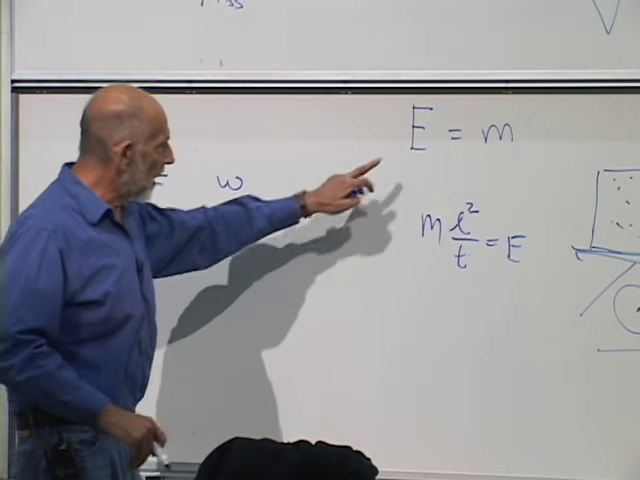
\includegraphics[width=0.72\textwidth]{lecture_01_figure_05.png}
\caption{En unidades con \(c=1\), la energía en reposo de un objeto masivo en reposo es \(E=m\).}
\lectureframe{01:25:40}
\end{figure}

Estas fórmulas parecen similares, pero significan cosas distintas. En \(E_{\mathrm{rest}}=m\), \(E\) es la energía en reposo de un objeto masivo. El fotón no tiene masa y no puede ponerse en reposo, así que su energía no es energía en reposo. La relación \(E_\gamma=\omega\) da la energía de un cuanto sin masa que está en movimiento.

\begin{classroomqa}
\lecturetimestamp{01:26:07}
\audiencequestion{¿Qué significa \emph{en reposo} si el reposo siempre es relativo a algo y el propio laboratorio no está absolutamente en reposo?}
\lecturerresponse{El reposo se define con respecto a un sistema de referencia elegido. Si una taza está inmóvil con respecto al laboratorio, entonces, en el sistema de referencia del laboratorio, su energía es su masa cuando \(c=1\), sin contribución cinética global. Otro observador que pase junto a la taza le atribuye también energía cinética. En general, distintos observadores atribuyen energías distintas al mismo objeto o fotón; la energía depende del sistema de referencia, y no hace falta afirmar que exista un reposo absoluto.}
\end{classroomqa}

Ahora se puede reconsiderar la convención de frecuencia angular. Escribir \(E_\gamma=\hbar\omega\) resulta compacto, pero antes \(\omega=2\pi f\) introdujo un factor de \(2\pi\).

\begin{classroomqa}
\lecturetimestamp{01:28:13}
\audiencequestion{¿Por qué usar la frecuencia angular \(\omega\), medida en radianes por segundo, en vez del número aparentemente más sencillo de ciclos completos por segundo?}
\lecturerresponse{La elección se debe en parte a razones históricas, y la respuesta matemática es práctica, aunque no inmediata. La respuesta que se propone aquí es provisional: escribir una vez las ecuaciones pertinentes con \(f\) y otra con \(\omega\), y luego ver qué convención deja menos factores de \(2\pi\). No se pueden hacer desaparecer los factores de \(2\pi\) en todas partes. También se sugirió una posible relación con la notación exponencial compleja, pero no se desarrolla aquí.}
\end{classroomqa}

\begin{classroomqa}
\lecturetimestamp{01:29:51}
\audiencequestion{¿Se pueden acelerar dos partículas hasta que su interacción gravitatoria mutua se vuelva importante?}
\lecturerresponse{En principio, sí. En la práctica, los aceleradores actuales están extraordinariamente lejos de ese régimen. La respuesta también depende de qué se entienda por partícula: un cuerpo macroscópico que gravita no es el caso de partícula elemental que nos ocupa.}
\end{classroomqa}

\begin{classroomqa}
\lecturetimestamp{01:30:27}
\audiencequestion{¿Qué puede servir como fuente de positrones?}
\lecturerresponse{Las colisiones de alta energía pueden crear positrones. Algunos procesos y desintegraciones nucleares también los producen.}
\end{classroomqa}

\begin{classroomqa}
\lecturetimestamp{01:30:53}
\audiencequestion{¿Se están usando aquí el tiempo y la distancia de Planck como unidades naturales?}
\lecturerresponse{No. Las unidades de Planck se obtienen al fijar \(G\), \(c\) y \(\hbar\) iguales a uno. La longitud de Planck resultante es muchísimo menor que las escalas de longitud de la física de partículas ordinaria, por lo que no es una escala práctica para medir aquí. Estas unidades son naturales cuando la gravedad, la mecánica cuántica y la relatividad son relevantes a la vez, como en la física de los agujeros negros, la cosmología o la gravedad cuántica. Cuando la gravedad es despreciable, resulta más útil fijar solo \(c\) y \(\hbar\) iguales a uno.}
\end{classroomqa}

\section{Momento, luz y resolución}

El siguiente concepto básico es el momento lineal. Un objeto en reposo no tiene momento, aunque su energía en reposo \(mc^2\) sea distinta de cero. Cuando se mueve, por lo general lleva momento. El momento se conserva en una colisión, al igual que la energía: cuando dos objetos chocan, el momento vectorial total antes y después del choque es el mismo. Todo aquello que esté sujeto a una ley de conservación merece especial atención.

El momento es un vector: apunta en la dirección del movimiento. Para un objeto no relativista,
\begin{equation}
\mathbf p=m\mathbf v.
\end{equation}
Esta no es la fórmula general de la relatividad y no se puede aplicar directamente a la luz.

Sin embargo, la luz lleva tanto momento como energía. La luz ordinaria ejerce un empuje tan pequeño que cuesta advertir su momento, pero un pulso láser intenso puede transferir un impulso considerable. Por ejemplo, el gran láser de Livermore puede impulsar material hacia dentro gracias al momento que transporta su radiación.

Consideremos un pulso suficientemente colimado, de modo que sus rayos viajen casi a lo largo de un mismo eje. Un haz real puede tener cierta dispersión angular, con partes que viajan en direcciones ligeramente distintas, pero, para un haz ideal colimado, el momento apunta a lo largo del haz y su módulo es
\begin{equation}
p=\frac{E}{c},
\qquad\text{or equivalently}\qquad
E=cp.
\end{equation}
Aquí se toma esta relación como un hecho relativista, en lugar de demostrarla. La siguiente comprobación dimensional solo confirma que sus unidades coinciden con las del momento ordinario:
\begin{equation}
\left[\frac{E}{c}\right]
=
\frac{M L^2 T^{-2}}{L T^{-1}}
=
M L T^{-1}
=
[m v]
=
[p].
\end{equation}
Esta comparación dimensional no atribuye una masa en reposo a la luz. El fotón tiene masa nula; lleva momento porque lleva energía y se mueve a \(c\).

La dirección de \(\mathbf p\) es la dirección de propagación. Su módulo suele ser difícil de detectar porque \(c\) aparece en el denominador. Un haz puede revelar fácilmente su energía al calentar o evaporar materia, mientras que el empuje mecánico que ejerce es mucho menor. Sin embargo, con suficiente intensidad ese empuje puede llegar a ser grande.

Para un fotón,
\begin{align}
p_\gamma
&=\frac{E_\gamma}{c}\\
&=\frac{\hbar\omega}{c}.
\end{align}
Para expresar esto en términos de longitud de onda, volvamos con cuidado a las relaciones de onda. Como
\begin{equation}
f\lambda=c,
\qquad
\omega=2\pi f,
\end{equation}
la relación correcta es
\begin{equation}
\omega\lambda=2\pi c,
\qquad
\omega=\frac{2\pi c}{\lambda}.
\end{equation}
Es fácil invertir el factor de \(2\pi\) si no se escriben las definiciones. Partamos otra vez de \(f\lambda=c\) y \(f=\omega/(2\pi)\) para despejar la cuestión:
\begin{equation}
\frac{\omega}{2\pi}\lambda=c
\quad\Longrightarrow\quad
\omega\lambda=2\pi c.
\end{equation}
Al sustituir, se obtiene
\begin{align}
p_\gamma
&=\frac{\hbar}{c}\frac{2\pi c}{\lambda}\\
&=\frac{2\pi\hbar}{\lambda}\\
&=\frac{h}{\lambda}.
\end{align}

\begin{classroomqa}
\lecturetimestamp{01:42:38}
\audiencequestion{¿Es \(2\pi\hbar\) igual a \(h\)?}
\lecturerresponse{Sí. Por definición, \(h=2\pi\hbar\), así que \(p_\gamma=2\pi\hbar/\lambda\) es lo mismo que \(p_\gamma=h/\lambda\). El factor \(2\pi\) vuelve a aparecer en algún sitio, sea cual sea la convención de frecuencia elegida.}
\end{classroomqa}

Cuanto menor es la longitud de onda, mayor es el momento del fotón. Un fotón de radio tiene una longitud de onda muy grande y un momento diminuto. Un fotón de rayos gamma tiene una longitud de onda muy corta y produce un impulso mucho mayor. Un solo fotón sigue produciendo apenas un pequeño impulso macroscópico, pero su momento es mucho mayor que el de un fotón de radio. Su energía también es mayor, ya que \(E_\gamma=cp_\gamma\).

Esta relación explica por qué los objetos más pequeños requieren máquinas más grandes. Una fotografía tomada con longitudes de onda mucho mayores que la cabeza de una persona solo mostraría una mancha borrosa. Para distinguir los rasgos faciales, la longitud de onda debe ser menor que la cabeza. Para resolver un pelo, debe ser comparable al grosor del pelo o menor. Para resolver la estructura de un átomo, la longitud de onda de la sonda no debe superar el tamaño del átomo:
\begin{equation}
\lambda_{\mathrm{probe}}\lesssim
\text{size of the structure to be resolved}.
\end{equation}
Por tanto, las estructuras más pequeñas requieren longitudes de onda más cortas, y las longitudes de onda más cortas requieren mayor momento y energía. La sonda no tiene por qué ser un fotón; las partículas de otros tipos y de alta energía obedecen la misma relación cuántica entre longitud de onda y momento. Para producirlas, se necesitan aceleradores que transfieran cada vez más energía a cada partícula. El par \(p_\gamma=h/\lambda\) y \(E_\gamma=\hbar\omega\) expresa el argumento: al aumentar la energía de la sonda, aumenta su momento y se acorta su longitud de onda.

Este ha sido el patrón recurrente de la física de partículas durante aproximadamente un siglo: mayor energía, mayor momento, menor longitud de onda y resolución espacial más fina.

\begin{classroomqa}
\lecturetimestamp{01:46:57}
\audiencequestion{¿Existe un límite inferior teórico para la longitud de onda?}
\lecturerresponse{Es posible. Se espera que ocurra algo nuevo cerca de la longitud de Planck, pero la respuesta es provisional. Si la resolución espacial tiene allí un límite inferior, esa escala sigue estando unos diecisiete órdenes de magnitud por debajo de las distancias que se exploran en el LHC; por tanto, los experimentos actuales todavía están enormemente lejos de ella.}
\end{classroomqa}

La misma línea de razonamiento sugiere una relación aproximada entre la escala de un acelerador y la escala que puede resolver.

\begin{classroomqa}
\lecturetimestamp{01:48:02}
\audiencequestion{¿La longitud de onda, o el tamaño que se puede resolver, es aproximadamente inversamente proporcional al tamaño del acelerador?}
\lecturerresponse{A grandes rasgos, sí, siempre que los campos eléctricos máximos que aceleran las partículas y los campos magnéticos que las guían sigan limitados por el aparato disponible. El gradiente de aceleración es la ganancia de energía por unidad de longitud. Para un acelerador lineal de longitud \(L\) y gradiente aproximadamente constante \(\mathcal G\),
\[
E_{\mathrm{beam}}\sim \mathcal G L.
\]
A energías ultrarrelativistas, la longitud de onda que se puede resolver es inversamente proporcional a la energía, de modo que aumentar la longitud del acelerador lineal mejora la resolución aproximadamente en el factor inverso. Se trata solo de una ley de escala heurística, no de una ley exacta. En las máquinas circulares, las partículas pueden recorrer repetidamente el mismo aparato, pero las cargas aceleradas emiten radiación al curvarse y pierden energía.}
\end{classroomqa}

\begin{classroomqa}
\lecturetimestamp{01:49:47}
\audiencequestion{¿Qué tamaño tendría que tener un acelerador para alcanzar la longitud de Planck?}
\lecturerresponse{Según esta escala aproximada, tendría que ser unos diecisiete órdenes de magnitud más largo que el acelerador del CERN. No tendría el tamaño del universo, pero sí aproximadamente una escala galáctica.}
\end{classroomqa}

\begin{classroomqa}
\lecturetimestamp{01:50:09}
\audiencequestion{¿Cómo se comparan las energías de los rayos cósmicos de mayor energía con las energías de los colisionadores?}
\lecturerresponse{Los rayos cósmicos individuales pueden tener mucha más energía en el laboratorio. Para hacer la comparación numérica, consideremos un rayo cósmico extremo con una energía en el laboratorio del orden de \(10^{21}\,\mathrm{eV}=10^{12}\,\mathrm{GeV}\). Pero un rayo cósmico choca contra un blanco que está en reposo en el laboratorio, mientras que un colisionador hace chocar de frente dos haces energéticos. Más importante aún, los experimentos útiles requieren flujo: muchas partículas y muchas colisiones bien controladas. Un rayo cósmico aislado puede no alcanzar el blanco pertinente o producir un suceso del que se pueda inferir poco. Una estimación deliberadamente extravagante, expresada en equivalente de petróleo, calculó que el suministro necesario para operar un acelerador galáctico útil sería de unos cien billones de barriles de petróleo por segundo. El objetivo de esa estimación es mostrar que obtener estadísticas de colisión suficientes sería un obstáculo tan grave como la longitud del acelerador, o incluso más.}
\end{classroomqa}

\editorialnote{La estimación en equivalente de petróleo es inconsistente en la fuente. Primero se enuncia y luego se repite como unos \(10^{14}\) barriles por segundo; una reformulación posterior da \(10^{11}\) barriles por segundo. Se conservan ambas magnitudes en lugar de conciliarlas en silencio.}

Estas son escalas de distancia reales, no meramente formales. El problema práctico es cómo explorarlas sin construir un acelerador galáctico ni suministrarle su energía fantástica.

\begin{classroomqa}
\lecturetimestamp{01:52:55}
\audiencequestion{¿Cómo debe compararse la energía del LHC con la de un rayo cósmico de energía \(10^{12}\,\mathrm{GeV}\)?}
\lecturerresponse{Para un proyectil ultrarrelativista con energía en el laboratorio \(E_{\mathrm{lab}}\) que choca contra un blanco fijo de masa \(m_{\mathrm{target}}\), la energía del centro de masas se comporta, en cuanto a su dependencia de las magnitudes, como
\[
E_{\mathrm{cm}}\simeq
\sqrt{2m_{\mathrm{target}}c^2E_{\mathrm{lab}}}.
\]
\editorialnote{La expresión mostrada para el blanco fijo hace explícita la dependencia de raíz cuadrada mencionada en el intercambio.}
Si se mantiene fija la masa del blanco, la energía útil de la colisión crece, por tanto, solo como la raíz cuadrada de la energía del proyectil. Así, un rayo cósmico de \(10^{12}\,\mathrm{GeV}\) corresponde, en orden de magnitud, a energías del orden de \(10^6\,\mathrm{GeV}\) por haz para haces que se propagan en sentidos opuestos, y no de \(10^{12}\,\mathrm{GeV}\) para cada haz. Los rayos cósmicos aún pueden superar las energías de los colisionadores terrestres, pero su flujo muy bajo hace impracticables los experimentos sistemáticos y controlados.}
\end{classroomqa}